\documentclass[answers,addpoints]{exam}
\usepackage[margin=10mm]{geometry}
\usepackage{amsthm}
\usepackage{float} %  figure inside minipage 
\usepackage{ifthen,empheq}
\usepackage[]{graphicx}
\usepackage[]{minted}
\usepackage{amssymb}
\usepackage[multidot]{grffile}
\usepackage{pgfplots}
\usepackage{pgfplotstable}
\setlength{\headheight}{20pt}

\usepackage{tikz}
\usepgfplotslibrary{external}
\tikzexternalize[prefix=_tikz/,shell escape=-shell-escape]
\tikzset{external/system call={pdflatex \tikzexternalcheckshellescape -halt-on-error -interaction=batchmode -jobname "\image" "\texsource"}}
\immediate\write18{mkdir -p _tikz}

\title{Solution to HW1}
\author{Dilawar Singh}
\usepackage{hyperref}

\begin{document}
\Large
\maketitle

\begin{questions}
\question{}
\begin{parts}

    \part[2] If $0<a<b$, and c is any real number, rewrite the sets $\{x: a<|x-c|<b\}$ in
    terms of intervals.   Do the same for $a=0$, and also give a clear description
    in words.  In this case, it will be something like "all the numbers between
    [something] and [something else] except for [these one(s)]

    \begin{solution}

        Its usually a good idea to play with concrete numbers before manipulating the
        symbols. For example, which one is correct  $a < b < c$ then $-a > -b > -c$, or
        $a < b < c$ then $-a < -b < -c$  etc. This become easy to answer once we notice
        that $1 < 2 < 3$ then $ -1 > -2 > -3$. This is just a quick and dirty reality
        check rather than replacement of understanding by doing proof. We are going to
        use this simple fact.

        We have, $ \{ x : a < | x - c | < b \}$ which means $a < x - c < b,
        \text{when}\; x > c$, and $a < c - x < b, \text{when}\; x < c$. The later can
        be rewritten as $-a > x -c > -b$. 

        For two different cases ($x > c$, and $x < c$), we have the following:
        \begin{align}
            a &< x - c < b  &(a + c < x < b + c) \\
            -a &> x -c < -b &(-a +c < x < -b +c)
        \end{align}

        Now we can use {\bf intervals } to rewrite it i.e. $x = { (a+c, b+c) \cup
        (-a+c,-b+c) }$.

        \begin{figure}[H]
            \foreach \fileindex in {1,...,4} {
                \tikzsetnextfilename{1a\fileindex}
                \begin{tikzpicture}[ ]
                ]
                \begin{axis}[
                        , xlabel=x,ylabel=$a < |x-c| <b$
                        , grid style={draw=gray!20}, grid = both, minor tick num = 0
                        , ymin = 0.5, ymax=1.5
                        , ytick={}, yticklabels={}
                        , domain=-1000:1000
                        , samples = 10000
                        , height = 5cm
                        , width = 8cm
                        , legend columns=-1
                    ]
                    \pgfmathsetseed{\number\pdfrandomseed} 
                    \pgfmathparse{100*rnd}\edef\a{\pgfmathresult}
                    \pgfmathparse{100*rand}\edef\c{\pgfmathresult}
                    \pgfmathparse{\a+100*rnd}\edef\b{\pgfmathresult}
                    \addplot[ only marks, domain=-1000:1000] gnuplot [ ] { 
                            \a< abs(x-\c) && abs(x-\c) < \b ? 1 : -1
                        };
                    \legend{a=\a; b=\b; c=\c}
                \end{axis}
            \end{tikzpicture}	
        }
        \caption{Numerical solution to problem 1(a)}
        \label{fig:1a}
    \end{figure}

    \end{solution}


    \part[2]
    Given $a<b$ real numbers, describe the intervals $(a,b)$ using the
    absolute value function.  That is, write $(a,b)=\{x:  ... \}$ where "$\ldots$"
    is some condition using absolute value.

    \begin{solution}

        $(a, b) = \{ x : x > a\; \text{and}\; x < b \}$. How about this,
        $ (a, b) = \{ x  : \left| x - \frac{a+b}{2} \right| < \frac{b-a}{2} \}$.

    Or better, since absolute value  $|x-y|$ denotes the distance between $x$ and
    $y$, we can say that for any $x$, $a\le x\ge b$, the distance between $x$
    and $a$ is aways less than distance between $b$ and $a$ i.e. $\{ x: |x-a|
        \le |a-b| \}$.  

        \tikzsetnextfilename{between}
        \begin{tikzpicture}[scale=1
                , every node/.style={ draw,circle, inner sep=1pt}
            ]
            \node[label=a] (a) at (0,0) {};
            \node[label=x] (x) at (1,0) {};
            \node[label=b] (b) at (3,0) {};
            \draw[-] (0,0) -- (1,0) -- (3,0);
        \end{tikzpicture}	

    \end{solution}

    \part[2] Similarly, express $\{a,b\}$, i.e. the set containing precisely the two
    (different) numbers a and b (e.g. $\{-14.7, e+\pi\}$ or $\{1776,1947\}$ ) using
    absolute values. 

    \begin{solution}

        How about this  $ \{a, b \} = \{ x : |x-a||x-b|=0 \}$. Or in other
        words, $\{a, b\} = \{ x : |x-a| = 0,\; \text{and}\; |x-b| = 0 \}$.
        Similarly, $\{a, b\} = \{ x : |x-\frac{a+b}{2}| = |\frac{a+b}{2}|$.

    \end{solution}

\end{parts}

\question[5] {
    Show that for any $x, y$, $||x|-|y|| \le |x+y|$.  (This is a useful
    counterpart to the triangle inequality and requires a very similar analysis.)
}

\begin{solution} 

    The simulation shown in figure \ref{fig:2a} shows that it is true.

    % create a new table with 10 rows and columns 'x' and 'y':
    \pgfplotstablenew
    [
        % define how the 'new' column shall be filled:
        create on use/x/.style ={ create col/expr ={100*rand}},
        create on use/y/.style ={ create col/expr ={100*rand}},
        columns={x,y}
    ] {1000} \mydata
    % show it:
    %\pgfplotstabletypeset\mydata

    \begin{figure}[H]
        \centering
        \begin{tikzpicture}[scale=1 , every node/.style={} ]
            \begin{axis}[
                    xlabel=$||x|-|y||$,ylabel=$|x+y|$
                ]
                \addplot[ only marks, mark=*, color=blue ] table [
                        , x expr=abs(abs(\thisrowno{0}) - abs(\thisrowno{1}))
                        , y expr=abs(\thisrowno{0}+\thisrowno{1})
                    ] {\mydata};
            \end{axis}
        \end{tikzpicture}	
        \caption{ $|x+y|$ is always greater than equal to $||x|-|y||$. Each blue
            dot's y-axis value represents value of $|x+y|$ while its x-axis value is value of
            $||x|-|y||$ for 1000 random samples of $(x,y)$ between intervals of
            $(-100, 100)\times(-100,100)$. (All) Blue dots are  falling over line of slope 1.
            That means that function on  y-axis is
            larger than the function on x-axis  for those (all) value of (x, y).
        }
        \label{fig:2a}
    \end{figure}

    \begin{proof}
        \begin{align*}
            (x+y)^2 
            &= x^2 + y^2 + 2xy \\
            &\ge x^2 + y^2 - 2 |xy| && \text{trick: } xy \le |xy| \implies xy \ge -|xy| \\
            &= |x|^2 + |y|^2 - 2|x||y| \\
            &= (|x| - |y|)^2
        \end{align*}

        Therefore, if $(x+y)^2 \ge (|x|-|y|)^2$, then,  $|x+y| \ge ||x|-|y||$.
        Recall that if $x^2 \ge y^2 \implies |x| \ge |y|$.

    \end{proof}

\end{solution}

% Problem 3
\question[5] {
    Write the set $\{x: |x^2-2x-3|>x\}$ as a union of intervals (i.e. figure out
    explicitly for which x this statement is true)
}

\begin{solution}

    First, lets see for what values of $x$, we have $x^2 - 2x - 3$ positive or
    negative. We have $(x-3)(x+1)$ as factors. So for $(-\infty, -1] \cup [3,
    \infty)$ it is positive and for rest, its negative.

    For the positive case $ x^2 - 3x - 3 > 0$ and for negative we have $ - x^2 + x
    + 3 > 0$. Solve for both cases and check if solution lies in the intervals
    computed before.

    Following figure shows probably correct answer. 
    \begin{figure}[H]
        \tikzsetnextfilename{sol3}
        \begin{tikzpicture}[scale=1]
            \begin{axis}[
                    xlabel=x,ylabel=$|x^2-2x-3|>x$
                    , grid style={draw=gray!20}, grid = both, minor tick num = 1
                    , ymin = 0, ymax= 2
                    , yticklabels = {}
                    , domain=-5:5
                    , samples=1000
                ]
                \addplot [only marks,color=blue] gnuplot  [ ] {
                        abs(x^2-2*x-3) > x ? 1 : -1
                    };
            \end{axis}
        \end{tikzpicture}
        \begin{tikzpicture}
            \begin{axis}[
                    domain=-5:5, samples = 1000
                    , ymin=-10, ymax=40
                ]
                \addplot [color=blue!50] { x^2 - 2*x - 3 };
                \addplot [color=blue] { x^2 - 3*x - 3 };
                \addplot [color=blue] { -x^2 - x + 3 };
                \addplot[color=red] coordinates { (-5,0) (-0.7928,0) };
                \addplot[color=red] coordinates { (3.7912,0) (5,0) };
                \addplot[color=red,thick] coordinates { (-1,-10) (-1,40) };
                \addplot[color=red,thick] coordinates { (3,-10) (3,40) };
                \legend{$x^2-2x-3$,$x^2-3x-3$,$x^2+x+3$}
            \end{axis}
        \end{tikzpicture}	
        \caption{On the left, interval for which given equation is true. On the
        right, geometrical interpretation}
    \end{figure}

\end{solution}


%% Problem 4
\question[14] {For each function $f:S \rightarrow T$, determine whether $f$
is one-to-one, onto, neither, or both. No explanation is needed. }

\begin{parts}

\part[2] $f : (0,\infty) \rightarrow (0,\infty), f(x) = 1/x$

\begin{solution}
   \tikzsetnextfilename{4a}
   \begin{tikzpicture}[scale=1
       , every node/.style={}
       ]
       \begin{semilogyaxis}[
           xlabel=x,ylabel=$1/x$
           , grid style={draw=gray!20}, grid = both, minor tick num = 1
           , domain=1e-6:5, samples=1000
       ]
           \addplot [color=blue] gnuplot [  ] { 1/x };
       \end{semilogyaxis}
   \end{tikzpicture}	
   one-to-one and onto. 
\end{solution}

\part[2] $g : \mathcal{R}\setminus\{0\} \rightarrow \mathcal{R}\setminus
\{0\},\; g(x) = 1/x$
\begin{solution}
   \tikzsetnextfilename{4b}
   \begin{tikzpicture}[scale=1
       , every node/.style={}
       ]
       \begin{axis}[
           xlabel=x,ylabel=$1/x$
           , grid style={draw=gray!20}, grid = both, minor tick num = 1
           , domain=-2:2, samples=1020
       ]
           \addplot [only marks,color=blue] gnuplot [  ] { 1/x };
       \end{axis}
   \end{tikzpicture}	
   One-to-one and onto.
\end{solution}

\part[2] $h:(0,\infty) \rightarrow (0, \infty), \; h(x) = 1/x^2$
\begin{solution}
   \tikzsetnextfilename{4c}
   \begin{tikzpicture}[scale=1
       , every node/.style={}
       ]
       \begin{axis}[
           xlabel=x,ylabel=$1/x$
           , grid style={draw=gray!20}, grid = both, minor tick num = 1
           , domain=0:3, samples=1020
       ]
           \addplot [color=blue] gnuplot [  ] { 1/(x^2)};
       \end{axis}
   \end{tikzpicture}	
    one-to-one and onto.
\end{solution}

\part[2] $k : \mathcal{R}\setminus\{0\} \rightarrow \mathcal{R}\setminus
\{0\},\; k(x) = 1/x^2$
\begin{solution}
    not one-to-one and not onto. Because there are negative values in co-domain
    for which there is no $x$ in domain. More than one x have same $1/x^2$ values.

    \begin{tikzpicture}[scale=1]
        \begin{axis}[
                xlabel=x,ylabel=$1/x^2$
        , grid style={draw=gray!20}, grid = both, minor tick num = 4 
        , domain=-1:1
        , samples = 100
        %, restrict y to domain=-10:1000
        ]
        \addplot [color=blue] { 1/(x^2) };
        \end{axis}
    \end{tikzpicture}
    
\end{solution}

\part[2] $l:[0,\pi/2] \rightarrow [-1,1],\; l(x) = sin(x)$

\begin{solution}
    one-to-one but not onto. Since there is no $x$ for which $sin x$ is
    negative.
    \begin{tikzpicture}[scale=1]
        \begin{axis}[
                xlabel=x(degree),ylabel=sin(x)
            , grid style={draw=gray!20}, grid = both, minor tick num = 1
            , domain=0:90
            , samples = 100
        ]
        \addplot [color=blue]{ sin(x) };
        \end{axis}
    \end{tikzpicture}
    
\end{solution}

\part[2] $m:(0,\pi/2) \rightarrow [-1,1],\; m(x)=sin(x)$
\begin{solution}
    Same as before.
\end{solution}

\part[2] $n:(0,\infty) \rightarrow (0,\infty),\; h(x)=\frac{1}{x^2+1}$    
\begin{solution}
    one-to-one but not onto. There is no $x$ for which $h(x)$ is $>1$.
    \begin{tikzpicture}[scale=1]
        \begin{axis}[
            xlabel=x,ylabel=$\frac{1}{1+x^2}$
            , grid style={draw=gray!20}, grid = both, minor tick num = 4 
            , domain=0:10
            , samples = 1000
        ]
            \addplot [color=blue] { 1/(x^2+1) };
        \end{axis}
    \end{tikzpicture}
    
    
\end{solution}

\end{parts}
% Problem 5.
\question[6] {
    Describe each set as a (union of) interval(s) or as an explicit finite of
    numbers, as appropriate 
}

\begin{parts}

    \part[2] $\{ x \in \mathcal{R}: 3x + 7 = 0 \}$
    \begin{solution}
        $ x = \{ \frac{-7}{3} \} $
    \end{solution}

    \part[2] $\{ x \in \mathcal{R}: \exists a\; \text{such that}\; 3x + 7 = a \}$ 
    \begin{solution}
        $ x = \left\{ x : \frac{a-7}{3} \right\} =
        \mathcal{R}$.  One to one and onto!
    \end{solution}

    \part[2]  $\{ x \in \mathcal{R}: \exists a\; \text{such that}\; a^2 - 2a = x \}$ 
    \begin{solution}
    $a = 1 \pm \sqrt{ 1 + x}$. For $a$ to be real, $x \ge -1
        \}$.

        Answer: $\bf [-1, \infty) $
    \end{solution}
\end{parts}


%% Problem 5.
\question[10]
\begin{parts}
\part[2] $|x-1| = |x-2|$ 
\begin{solution}
    We plot the function $|x-1|-|x-2|$ and find the place where it becomes
    zero. Following is geometrical picture.

    \begin{tikzpicture}[scale=1]
        \begin{axis}[
                xlabel=x,ylabel=$|x-1|-|x-2|$
                , domain=-100:100
                , grid style={draw=gray!20}, grid = both, minor tick num = 4 
            ]
            \addplot [color=blue] { abs(x-1) - abs(x-2) };
            \addplot [color=red] { 0 };
        \end{axis}
    \end{tikzpicture}
    \[   
        |x-1|-|x-2| = 
        \begin{cases}
            x \ge 2 & x-1-x+2 = 1 \\ 
            1 \le x < 2 & x-1-2+x = 2x-3\\
            x < 1 &  1-x-2-x = -1\\
        \end{cases}
    \]

    Answer: $\bf 3/2$.
\end{solution}

\part[2] $x^2+4|x|+3 = 0$
\begin{solution}

    \begin{tikzpicture}[scale=1]
        \begin{axis}[
                xlabel=x,ylabel=$x^2+4|x|+3$
                , grid style={draw=gray!20}, grid = both, minor tick num = 1
                , samples = 1000
            ]
            \addplot [color=blue] { x^2+4*abs(x)+3 };
            \addplot [color=red] {  0 };
        \end{axis}
    \end{tikzpicture}
    Answer: $\bf \{\} $

\end{solution}

\part[2] $x^2-4|x|-3 = 0$
\begin{solution}

    \begin{tikzpicture}[scale=1]
        \begin{axis}[
                xlabel=x,ylabel=$x^2-4|x|-3$
                , grid style={draw=gray!20}, grid = both, minor tick num = 1
                , samples = 1000
            ]
            \addplot [color=blue] { x^2-4*abs(x)-3 };
            \addplot [color=red] {  0 };
        \end{axis}
    \end{tikzpicture}

    Answer: $\bf \{ \frac{-4-\sqrt{28}}{2}, \frac{4+\sqrt{28}}{2} \} $

    {\bf Note} Previous equation looks like a fly butt and this one like a human
    butt.  A mere change of sign!

\end{solution}

\part[2] $|3x-1| < 0.1$
\begin{solution}
    \begin{tikzpicture}[scale=1]
        \begin{axis}[
                xlabel=x,ylabel=$|3x-1|$
                , ymax = 0.2
                , grid style={draw=gray!20}, grid = both, minor tick num = 1
                , domain=0:0.5
                , samples = 200
            ]
            \addplot [color=blue] { abs(3*x - 1) };
            \addplot [color=red] { 0.1 };
        \end{axis}
    \end{tikzpicture}

    Answer: $\bf (\frac{9}{30}, \frac{11}{30})$. 

\end{solution}

\part[2] $3 < \sqrt{2x+1} < 4$
\begin{solution}
    \begin{tikzpicture}[scale=1]
        \begin{axis}[
                xlabel=x,ylabel=$\sqrt{2x+1}$
                , grid style={draw=gray!20}, grid = both, minor tick num = 1
                , domain=0:10
            ]
            \addplot [color=blue] { (2*x + 1)^0.5 };
            \addplot [color=red] { 3 };
            \addplot [color=red] { 4 };
        \end{axis}
    \end{tikzpicture}

    Answer : $\bf( 4, 7.5) $


\end{solution}


\end{parts}



%% Problem 7. From Lang.
\question[8] {Problems from Lang, 3,4,6,13 (on page 8)}
\begin{parts}

\part[2] $|x^2-2| \le 1$
\begin{solution}

    \begin{tikzpicture}[scale=1
            , every node/.style={}
        ]
        \begin{axis}[
                xlabel=x,ylabel=$|x^2-2|$
                , xmin = -3, xmax = 3,
                , grid style={draw=gray!20}, grid = both, minor tick num = 1
            ]
            \addplot [color=blue] gnuplot [ raw gnuplot ] { plot abs(x^2-2) }; 
            \addplot [color=red] gnuplot [ raw gnuplot ] { plot 1 };
        \end{axis}
    \end{tikzpicture}	

    Answer: $\bf x = \left[ -\sqrt3, -1\right] \cup \left[1,\sqrt3\right]$

\end{solution}

\part[2] $|x-5| < |x+1| $
\begin{solution}

    \begin{tikzpicture}[scale=1]
        \begin{axis}[xlabel=x,ylabel=$|x-5|-|x+1|$
                , grid=both 
                , grid style = {draw=gray!10}
                , minor tick num = 4
                , domain=-10:10
                , samples = 1000
            ]
            \addplot [color=blue] gnuplot [  ] { abs(x - 5) - abs(x+1) };
            \addplot [color=red] gnuplot [ ] { 0 };
        \end{axis}
    \end{tikzpicture}

    Answer: $\bf (2, \infty)$.


\end{solution}

\part[2]  $(x+1)(x-1) > 0$ 
\begin{solution}
    The figure below shows the plot of this function. We are interested in values
    of $x$ for which the function is greater than 0 (red line).

    \begin{tikzpicture}[scale=1]
        \begin{axis}[xlabel=x,ylabel=(x+1)(x-1)
                , grid=both 
                , grid style = {draw=gray!10}
                , minor tick num = 4
            ]
            \addplot [color=blue] gnuplot [ raw gnuplot ] { plot (x+1)*(x-1) };
            \addplot [color=red] gnuplot [ raw gnuplot ] { plot 1 };
        \end{axis}
    \end{tikzpicture}

    Answer $\bf x = (1,\infty) \cup (-\infty,-1)$
\end{solution}

\part[2] $ (4x+7)^{20} (2x+8) < 0$ 
\begin{solution} 

    This is good example to demonstrate the limitation of numerical analysis. On
    the left, I've plotted the given function and it grows rapidly. It is hard to
    figure out exactly where this function goes negative. To overcome this, I
    have plotted the log value of function on the right. Things improves but the
    we run into numerical issues in the interval (-5, 0 ). Though, if we do a
    "mathematical analysis" of this problem, answer is easy to find.

    \begin{tikzpicture}[scale=1]
        \begin{axis}[
                xlabel=x,ylabel=$(4x+7)^{20}(2x+8)$
                , grid style={draw=gray!20}, grid = both, minor tick num = 4 
                %, xmin=0,xmax = 4
            ]
            \addplot [color=blue] gnuplot [ raw gnuplot ] { plot (4*x+7)^20*(2*x+8) };
            \addplot [color=red] gnuplot [ raw gnuplot ] { plot 0 };
        \end{axis}
    \end{tikzpicture}
    \begin{tikzpicture}
        \begin{axis}[
                xlabel=x,ylabel=$\log((4x+7)^{20}(2x+8))$
                , grid style={draw=gray!20}, grid = both, minor tick num = 4 
                %, xmin=0,xmax = 4
            ]
            \addplot [color=blue] gnuplot [ raw gnuplot ] { plot log((4*x+7)^20*(2*x+8)) };
            \addplot [color=red] gnuplot [ raw gnuplot ] { plot 1 };
        \end{axis}
    \end{tikzpicture}


    First term in the expression ($4x+7$) is raised to even powers.
    Its value will always be positive. We only have to worry about the case where
    $2x+8<0$.  

    Answer: $\bf x = (-\infty, -4)$.  


\end{solution}

\end{parts}

\end{questions}

\end{document}          
